\documentclass{article}
\usepackage{iclr2025_conference,times}
\iclrfinalcopy

\input{math_commands.tex}

\usepackage{hyperref}
\usepackage{url}
\usepackage{graphicx}
\usepackage{float}

\title{Analyzing Memorization in VAR-d16 with UnitMem}

\author{Wenzheng Tang}

\begin{document}

\maketitle
\lhead{}

\begin{abstract}
We apply UnitMem to pretrained VAR-d16 to locate its highest-scoring units and
identify the training images that activate them most selectively. Using
10{,}000 ImageNet training images and ten augmentations per image, we compute
UnitMem at each image-dependent generation scale and average the scores across
scales. Of the top 10\% of units, 92.1\% are located in fc1 layers and 56.9\%
occur in blocks 0--2. For each selected unit, we identify its most activating
training image at each scale. These responses concentrate on a small subset of
the data: 3.8\% of images account for half of all selections. Compared with
class-matched controls, the most frequently selected images have higher
Laplacian sharpness and require more JPEG bytes per pixel.
\end{abstract}

\vspace{-4pt}
\section{Introduction}
\label{sec:intro}
\vspace{-2pt}

VAR generates images autoregressively from coarse to fine scales
\citep{tian2024var}. Its Transformer reuses the same blocks at each generation
scale. UnitMem, originally proposed for self-supervised vision encoders,
quantifies a unit's image selectivity by comparing its response to the most
activating image with its mean response to all others
\citep{wang2024localizing}.

Kasliwal et al. adapted UnitMem to VAR by computing fc1 scores separately at
each generation scale \citep{kasliwal2025localizing}. Building on this
formulation, we ask: (1) which layer types and block depths contain the
highest-scoring 10\% of units; and (2) which training images activate these
units most strongly, and what properties distinguish them from class-matched
controls?

\vspace{-3pt}
\section{Method}
\label{sec:method}
\vspace{-2pt}

We evaluate pretrained VAR-d16 on a balanced subset of 10{,}000 ImageNet
training images (10 per class) \citep{russakovsky2015imagenet}, using teacher
forcing and ten augmentations per image. Following the scale-wise VAR formulation of UnitMem
\citep{wang2024localizing,kasliwal2025localizing}, the response of unit $u$ to
image $x$ at scale $s$ is its mean absolute activation over views and tokens:
\vspace{-2pt}
\[
a_{u,s}(x)=\frac{1}{10}\sum_{r=1}^{10}\frac{1}{|T_s|}
\sum_{t\in T_s}\left|h_{u,t}(x^{(r)})\right|.
\]
\vspace{-2pt}
UnitMem is computed independently at each scale by comparing the most
activating image with the mean response to the remaining images in $D'$:
\vspace{-2pt}
\[
\mathrm{UnitMem}_{u,s}=
\frac{\mu_{\max,u,s}-\mu_{-\max,u,s}}
     {\mu_{\max,u,s}+\mu_{-\max,u,s}}.
\]
\vspace{-2pt}

\textbf{RQ1.} We average the nine image-dependent scale scores,
$S_u=\frac{1}{9}\sum_{s=1}^{9}\mathrm{UnitMem}_{u,s}$, and jointly rank fc1,
attn.proj, and fc2 units from all 16 blocks. Scale 0 is excluded because it
contains only the class condition. We select the overall top 10\% and report
the fraction of each layer type and block entering this set, together with the
joint layer-type-by-block distribution.

\textbf{RQ2.} For each selected unit and scale, we record
$x^*_{u,s}=\arg\max_{x\in D'}a_{u,s}(x)$. Each unit-scale pair casts one vote,
and images are ranked by their total votes. We compare the top-50 images with
class-matched controls on eight predefined low-level features: grayscale
entropy, edge density, Laplacian sharpness, luminance contrast, mean
saturation, colorfulness, center-to-border contrast, and JPEG bytes per pixel.
We blindly annotated seven predefined patterns in a randomized contact sheet
of the top-50 images and 50 class-matched controls, with labels and votes hidden.
Class-matched permutation tests (class-stratified for annotations) and separate
BH-FDR corrections were used. Cohen's $d$ and $h$ measure effect sizes for
continuous features and binary patterns, respectively; $q$ denotes the
BH-FDR-adjusted $p$-value.

\begin{figure}[t]
\vspace{-4pt}
\centering
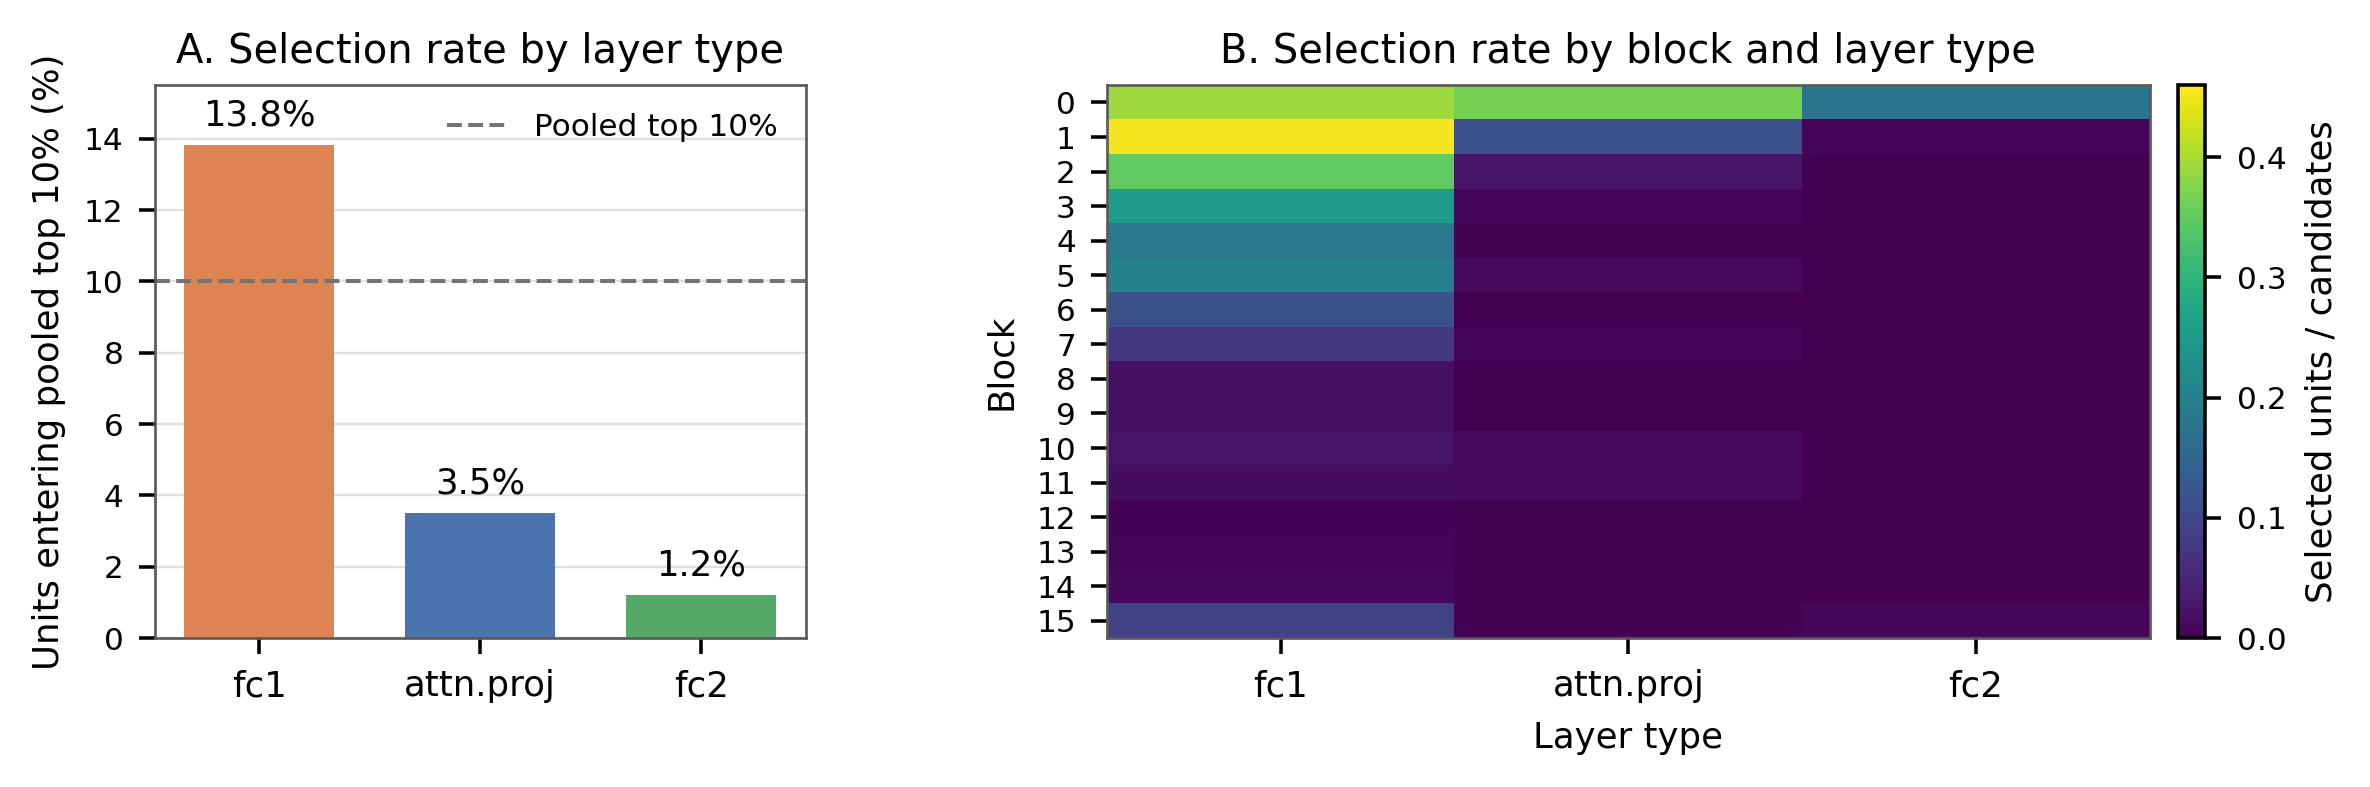
\includegraphics[width=0.92\linewidth]{fig1_rq1.png}
\vspace{-5pt}
\caption{Location of the overall top 10\% UnitMem units in VAR-d16:
\textbf{A} fraction of each layer type entering the pooled top decile;
\textbf{B} selection rate for each layer-type--block pair.}
\label{fig:rq1}
\vspace{-8pt}
\end{figure}

\vspace{-2pt}
\section{RQ1: Where Are the Highest-Scoring Units?}
\label{sec:rq1}
\vspace{-2pt}

\textbf{Layer type.} Fc1, attn.proj, and fc2 selection rates are 13.82\%, 3.51\%,
and 1.21\%; fc1 therefore accounts for 92.14\% of the 9{,}830 selected units.

\textbf{Block location.} Blocks 0--2 contain 56.93\% of selected units, with the
highest rate in block 1's fc1 layer (45.43\%). Rates generally decrease with
depth, followed by a smaller rise in block 15.

\vspace{-3pt}
\section{RQ2: Which Images Are Selected?}
\label{sec:rq2}
\vspace{-2pt}

\textbf{Vote distribution.} Of 10{,}000 images, 6{,}319 (63.19\%) receive a vote,
while 383 (3.83\%) account for half. The top 10/50 receive 9.39\%/21.69\% of all
votes. The most-selected image receives 2{,}188 unit-scale votes cast by 464
distinct units across 15 blocks, three layer types, and eight scales.

\textbf{Image properties.} Only Laplacian sharpness ($d=0.64$, $q=0.0008$)
and JPEG bytes per pixel ($d=0.43$, $q=0.0072$) remain significant after
BH-FDR correction; the other six features do not (all $q\geq0.135$).

\textbf{Semantic patterns.} Repetitive textures/geometric patterns (56\% vs.
28\%; $h{=}0.58$, $q{=}0.012$) and extreme close-ups/crops (46\% vs. 22\%;
$h{=}0.51$, $q{=}0.031$) were the only patterns enriched after BH-FDR; the
other five showed no reliable differences.

\vspace{-8pt}
\begin{figure}[H]
\vspace{-8pt}
\centering
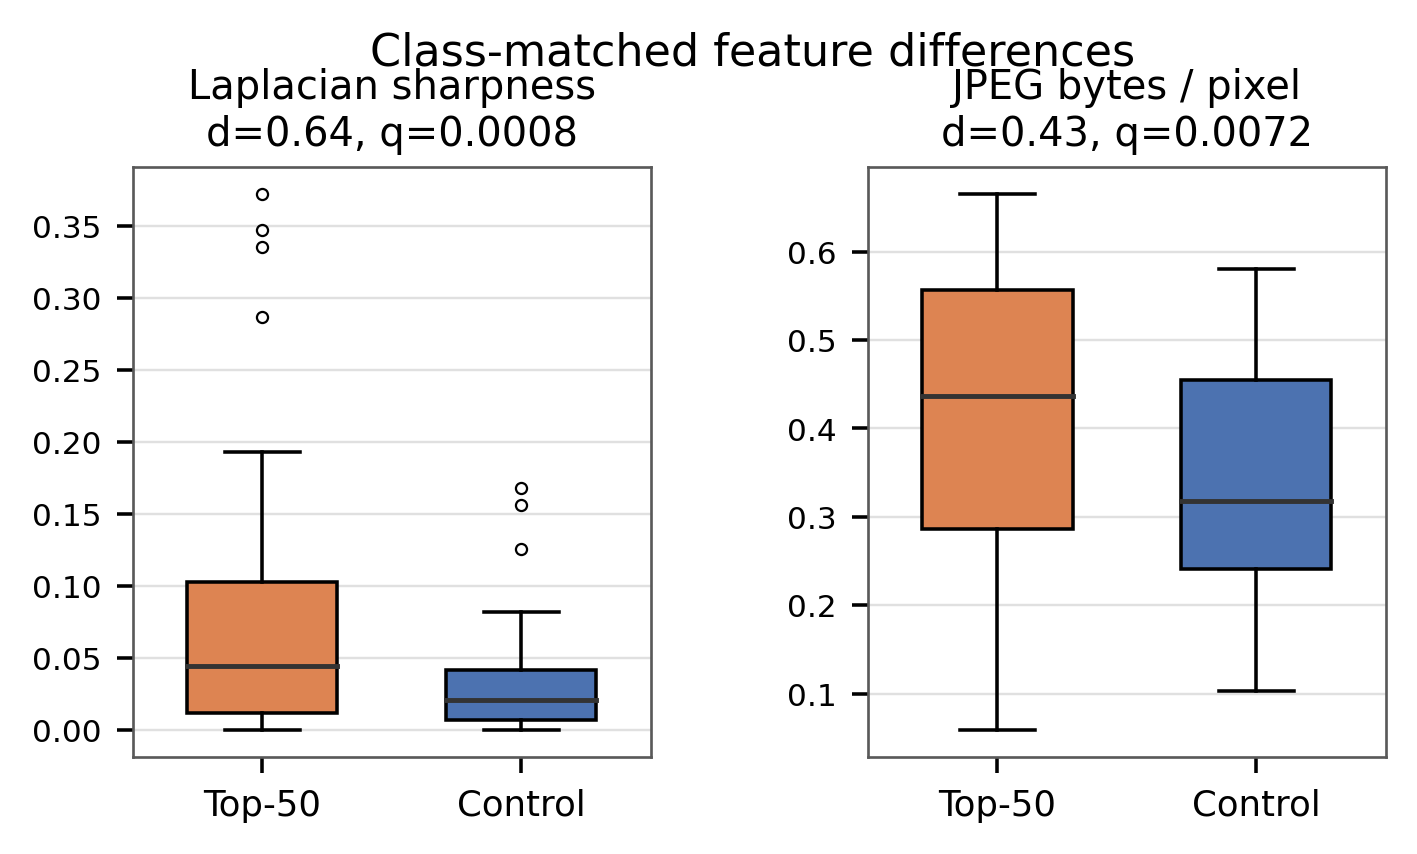
\includegraphics[width=0.46\linewidth]{fig2_rq2.png}
\vspace{-6pt}
\caption{RQ2 image features that differ from class-matched controls after
BH-FDR correction.}
\label{fig:rq2}
\vspace{-18pt}
\end{figure}

\vspace{-14pt}
\section{Conclusion}
\label{sec:conclusion}
\vspace{-4pt}

Equal averaging across the nine image-dependent scale scores places high-UnitMem
units mainly in early fc1 layers (92.1\% fc1; 56.9\% blocks 0--2). Selections are
concentrated (3.8\% of images receive half) and favor images with higher
Laplacian sharpness, more JPEG bytes per pixel, repetitive textures, and extreme
close-ups relative to class-matched controls.

\clearpage
\bibliography{refs}
\bibliographystyle{iclr2025_conference}

\end{document}
